%************************************************
\myChapter{Metoda}\label{ch:solution} % $\mathbb{ZNR}$
%************************************************

\section{Sprzęt}
W swojej pracy wykorzystałem sprzęt, który pokrótce omówię.

\subsection{Elementy}
Sprzęt, abstrahując od szczegółowego sposobu realizacji, składa się z dwóch \index{marker}markerów, których funkcje pełnią głośniki ultradźwiękowe, trzech \index{odbiornik}odbiorników pod postacią mikrofonów ultradźwiękowych oraz \index{mikrokontroler}mikrokontrolera \textsmaller{AVR Atmega8}. Dodatkowo w układzie zamontowanych jest 8 diod LED, które służą do nadzorowania stanu układu.

\subsection{W ogóle}
Działanie mikrokontrolera sprowadza się do ciągłego, aktywnego prowadzenia pomiarów opóźnień czasów propagacji sygnału ultradźwiękowego pomiędzy markerami, a odbiornikami. Pozyskane w ten sposób dane przekazywane są za pomocą specjalnie opracowanego \index{protokół}protokołu do komputera, gdzie następuje ich dalsza obróbka.

Uproszczony schemat układu prezentuje rysunek~\ref{fig:device_scheme}.

\begin{figure}
 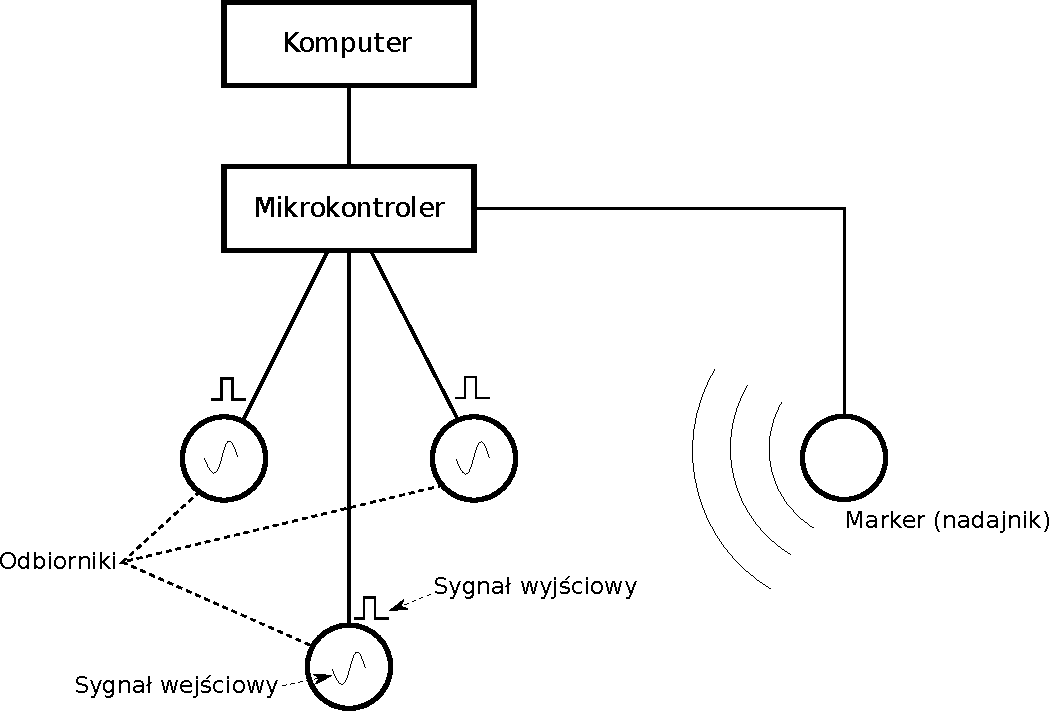
\includegraphics[width=\textwidth]{gfx/diagramy/schemat_blokowy_ukladu}
 \caption{Uproszczony schemat blokowy układu}
 \label{fig:device_scheme}
\end{figure}

\subsection{W szczególe}
Działanie systemu opiera się na założeniu, że dźwięk w powietrzu rozchodzi się ze stałą, znaną szybkością.\graffito{Założenie takie można przyjąć, gdyż odchylenia tej wartości spowodowane temperaturą i wilgotnością powietrza są niewielkie i nie wpływają znacząco na działanie systemu}

Ponieważ szybkość ta jest stała, można łatwo wyznaczyć odległość, jaką musiał przebyć dźwięk, aby dotrzeć do odbiornika:
\begin{equation}
 x = v \cdot t
 \label{eq:sound_distance}
\end{equation}
gdzie:\graffito{dodać informację nt. kalibracji - zmiana protokołu na obsługę potwierdzeń, oczekiwanie mikrokontrolera na potwierdzenie, rozpoczynanie kalibracją, wymóg piramidki do kalibracji}
\begin{description}
 \item[$x$] \ppauza~odległość przebyta przez dźwięk,
 \item[$v$] \ppauza~szybkość dźwięku w powietrzu\graffito{Przyjęto prędkość dźwięku w powietrzu $v = 340\frac{\textrm{m}}{\textrm{s}}$},
 \item[$t$] \ppauza~czas od wysłania sygnału do jego dotarcia do odbiornika. 
\end{description}

Dane, jakie przekazywane są do komputera w celu dalszej obróbki zawierają, poza specyfikacją \index{protokół}protokołu, tylko i wyłącznie odczyty z licznika dla każdego z odbiorników.

\paragraph{Przetwarzanie danych}
Aby dane były do czegoś użyteczne, wymagane jest ich przetworzenie. Przetwarzanie danych tej postaci może odbywać się różnorakimi metodami, np.:
\begin{itemize}
 \item rozpoznawanie gestów za pomocą sieci neuronowych,
 \item odtworzenie pozycji markera w trzech wymiarach,
 \item oczekiwanie na przemieszczenie markera do predefiniowanej pozycji,
 \item wiele innych.
\end{itemize}

\paragraph{Odtworzenie pozycji markera}
\index{marker}
W celach demonstracyjnych postanowiłem pokazać, jak odtworzyć pozycję markera w trzech wymiarach, korzystając tylko z informacji o względnym położeniu odbiorników oraz przekazywanych do komputera danych o czasie, w jakim sygnał z markera dotarł do każdego z tych odbiorników.
\newline

Aby wyznaczyć położenie markera w trójwymiarowej przestrzeni, mając do dyspozycji odległości od każdego z odbiorników, można założyć, że odbiorniki są środkami sfer, a promieniem każdej z nich \ppauza odległość, jaką przebył dźwięk od markera do tego odbiornika. Punkt przecięcia się tych sfer będzie pozycją markera.

\begin{figure}
  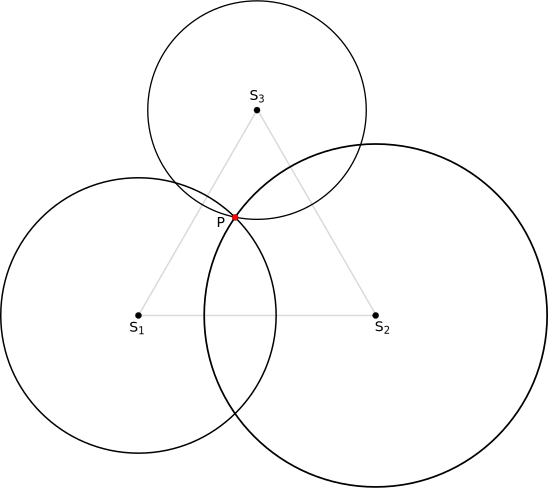
\includegraphics[width=\textwidth]{gfx/diagramy/schemat_przeciecia_sfer}
  \caption{Poglądowy schemat rozmieszczenia czujników}
  \label{fig:schema_spheres}
\end{figure}

\paragraph{Rozmieszczenie elementów}
Rysunek \ref{fig:schema_spheres}\graffito{W rysunku przyjęto widok ,,od przodu'', tzn. zachodzi $z = 0$ dla wszystkich elementów z wyjątkiem punktu $P$} prezentuje rozmieszczenie odbiorników na płycie testowej. Znajdują się one w punktach oznaczonych odpowiednio jako $S_1$, $S_2$ i $S_3$. Punkt $P$ to punkt przecięcia się sfer.

Ponieważ zastosowano tylko trzy \index{odbiornik}odbiorniki, będą one zawsze leżeć w jednej płaszczyźnie. Powoduje to, że będą istniały dokładnie dwa punkty przecięcia wspomnianych powyżej sfer \ppauza lustrzane do siebie względem płaszczyzny, w której znajdują się odbiorniki.\graffito{dodać notatkę w testach o możliwości wyeliminowania tego 'defektu' poprzez dodanie 4-tego odbiornika, niewspółpłaszczyznowego, jednak spowoduje to wzrost kosztów obliczeń}

Należy wziąć pod uwagę fakt, że zarówno marker jak i odbiorniki są urządzeniami ,,kierunkowymi'', umieszczonymi w tulejach, które powodują, że sygnał nie jest wysyłany dookólnie, lecz w pewnym \ppauza z grubsza określonym \ppauza kierunku, zaś amplituda sygnału odbieranego będzie większa, jeśli będzie on wpadał w tuleję, przez co szansa uznania go za poprawny jest znacznie większa.\graffito{sygnał dochodzący z boku może być ze słaby, aby został wyłapany}

Ta cecha układu została wykorzystana poprzez przeznaczenie układu do noszenia na tułowiu \ppauza łatwo zauważyć, że użytkownikowi ciężko byłoby przesunąć \index{marker}marker zbyt daleko do tyłu, gdyż ograniczałyby go stawy. 

Wykorzystując fakt, że człowiek trzyma ręce w większości przypadków przed sobą, szczególnie jeśli zamierza coś nimi robić, można spokojnie odrzucić jeden z punktów \ppauza ten który znajduje się ,,z tyłu''.

\paragraph{Trilateracja}
\label{par:trilateration}
\index{trilateracja}
Metoda wyznaczenia trójwymiarowej pozycji znając odległości od trzech punktów o znanych współrzędnych nazywana jest \textit{trilateracją}\graffito{dodać info skąd to wiadomo}.

Problem wyznaczenia położenia markera można uprościć, przyjmując określony układ współrzędnych, w którym jeden z odbiorników znajduje się w początku układu współrzędnych, drugi na osi $x$, a trzeci pozostaje ,,swobodny''\graffito{Współrzędna $z$ dla wszystkich odbiorników równa jest~$0$}. Rozmieszczenie takie zaprezentowano na rysunku \ref{fig:schema_coordinates}, odbiorniki mają współrzędne odpowiednio:
\begin{center}
 $S_1 (0, 0)$

 $S_2 (a, 0)$

 $S_3 (b, c)$
\end{center}

\begin{figure}
  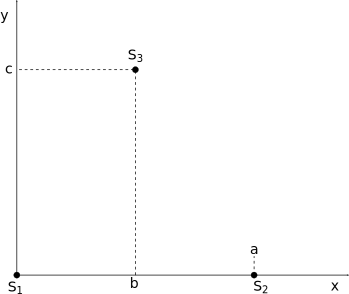
\includegraphics[width=\textwidth]{gfx/diagramy/schemat_uklad_wspolrzednych_clipped}
  \caption{Układ współrzędnych wykorzystany do określenia pozycji odbiorników}
  \label{fig:schema_coordinates}
\end{figure}

Równanie sfery ze środkiem w punkcie o współrzędnych $(x_0, y_0, z_0)$ i promieniu $r$ przyjmuje postać:
\begin{equation}
 r = \sqrt{(x - x_0)^2 + (y - y_0)^2 + (z - z_0)^2}
 \label{eq:sphere}
\end{equation}

Podstawiając do równania \ref{eq:sphere} współrzędne punktów $S_1$, $S_2$ i $S_3$ otrzymujemy następujący układ równań:
\begin{equation}
 \begin{cases}
  r_1 = \sqrt{x^2 + y^2 + z^2} \\
  r_2 = \sqrt{(x - a)^2 + y^2 + z^2} \\
  r_3 = \sqrt{(x - b)^2 + (y - c)^2 + z^2}
 \end{cases}
 \label{eq:sphere_system_1}
\end{equation}
gdzie $r_1$, $r_2$ i $r_3$ to odpowiednio odległości \index{marker}markera od każdego z \index{odbiornik}odbiorników \textsmaller{\#1}, \textsmaller{\#2} i \textsmaller{\#3}, a zarazem promienie sfer, których punktu przecięcia poszukujemy.

W celu uproszczenia następnych obliczeń przyjmijmy poniższą postać równania \ref{eq:sphere_system_1}\graffito{należy pamiętać, że promień jest zawsze nieujemny}:
\begin{equation}
 \begin{cases}
  r_1^2 = x^2 + y^2 + z^2 \\
  r_2^2 = (x - a)^2 + y^2 + z^2 \\
  r_3^2 = (x - b)^2 + (y - c)^2 + z^2
 \end{cases}
 \label{eq:sphere_system_2}
\end{equation}

Rozwińmy najpierw drugie równanie z układu \ref{eq:sphere_system_2}:
\begin{equation}
 r_2^2 = (x - a)^2 + y^2 + z^2 = x^2 - 2xa + a^2 + y^2 + z^2
\end{equation}

Następnie odejmijmy je od równania pierwszego z systemu \ref{eq:sphere_system_2}:
\begin{equation}
 r_1^2 - r_2^2 = x^2 + y^2 + z^2 - (x^2 - 2xa + a^2 + y^2 + z^2) = 2xa - a^2
 \label{eq:determine_x_1}
\end{equation}

Z równania \ref{eq:determine_x_1} można łatwo wyznaczyć $x$:
\begin{eqnarray}
 r_1^2 - r_2^2 = 2xa - a^2 & | & + a^2\\
 r_1^2 - r_2^2 + a^2 = 2xa & | & \colon 2a\\
 x = \frac{r_1^2 - r_2^2 + a^2}{2a} \label{eq:determine_x_2}
\end{eqnarray}
\graffito{jak zapisać działanie wykonywane stronami?}

Podstawiając $x$ z równania \ref{eq:determine_x_2} do pierwszego równania układu \ref{eq:sphere_system_2} dowiemy się, które punkty są wspólne dla sfer mających środki w odpowiednio\graffito{przecinki?} $S_1$ i $S_2$:

\begin{eqnarray}
 r_1^2 = x^2 + y^2 + z^2 \\
 r_1^2 = \left(\frac{r_1^2 - r_2^2 + a^2}{2a}\right)^2 + y^2 + z^2 \\
 y^2 + z^2 = r_1^2 - \left(\frac{r_1^2 - r_2^2 + a^2}{2a}\right)^2 \label{eq:intersection_circle}
\end{eqnarray}

W równaniu \ref{eq:intersection_circle} prawa strona jest stała, widać więc, że jest to równanie okręgu.

Rozwińmy teraz równanie trzeciej sfery:
\begin{eqnarray}
 r^2_3 & = & (x - b)^2 + (y - c)^2 + z^2 \label{eq:third_sphere} \\
       & = & x^2 - 2bx + b^2 + y^2 - 2cy + c^2 + z^2 \nonumber
\end{eqnarray}

Podstawiając równanie pierwszej sfery przekształcone do postaci
\begin{equation*}
 y^2 + z^2 = r_1^2 - x^2
\end{equation*}
do wzoru \ref{eq:third_sphere} otrzymujemy:
\begin{eqnarray}
r_3^2 & = & x^2 - 2bx + b^2 - 2cy + c^2 + r_1^2 - x^2 \label{eq:third_sphere_substituted} \\
      & = & -2bx + b^2 - 2cy + c^2 + r_1^2 \nonumber
\end{eqnarray}

Na podstawie równania \ref{eq:third_sphere_substituted} można wyznaczyć $y$:
\begin{eqnarray}
 r_3^2 = -2bx + b^2 - 2cy + c^2 + r_1^2 & | & +2cy - r_3^2 \\
 2cy   = -2bx + b^2 + c^2 + r_1^2 - r_3^2 & | & \colon 2c \\
 y     = \frac{-2bx + b^2 + c^2 + r_1^2 - r_3^2}{2c} & & \label{determine_y}
\end{eqnarray}

Ponieważ $x$ jest stałe\graffito{stałe i znane?}, jak pokazuje równanie \ref{eq:determine_x_2}, to prawa strona równania \ref{determine_y} również będzie stała.

Do wyznaczenia pozostało jeszcze jedynie $z$. Aby policzyć jego wartość, weźmy wzór pierwszej sfery z układu \ref{eq:sphere_system_1}, stąd $z$ będzie wynosić:
\begin{equation}
 z = \pm\sqrt{r_1^2 - x^2 - y^2}
\end{equation}

Jak jednak pamiętamy z opisu, jeden z tych punktów, ,,tylny'' odrzucamy, w związku z czym $z$ ostatecznie przyjmuje postać:
\begin{equation}
 z = \sqrt{r_1^2 - x^2 - y^2}
\end{equation}

Reasumując, jeśli przyjąć rozmieszczenie \index{odbiornik}odbiorników takie jak na rysunku~\ref{fig:schema_coordinates}, punkt przecięcia się sfer\graffito{Dla uproszczenia przyjmujemy, że punkt taki zawsze istnieje, co w skonstruowanym systemie jest prawdziwe} będzie miał następujące współrzędne:\graffito{dodać info o lokalności układu i konieczności jego odtworzenia}
\begin{eqnarray}
 x & = & \frac{r_1^2 - r_2^2 + a^2}{2a} \label{eq:trilateration_final_x}\\
 y & = & \frac{-2bx + b^2 + c^2 + r_1^2 - r_3^2}{2c} \label{eq:trilateration_final_y}\\
   & = & \frac{-b\frac{r_1^2 - r_2^2 + a^2}{a} + b^2 + c^2 + r_1^2 - r_3^2}{2c} \nonumber \\
 z & = & \sqrt{r_1^2 - x^2 - y^2} \label{eq:trilateration_final_z}\\
   & = & \sqrt{r_1^2 - \left(\frac{r_1^2 - r_2^2 + a^2}{2a}\right)^2 - \left(\frac{b\frac{r_1^2 - r_2^2 + a^2}{-a} + b^2 + c^2 + r_1^2 - r_3^2}{2c}\right)^2} \nonumber
\end{eqnarray}

Jako ciekawostkę warto dodać informację, że system \textsc{GPS} korzysta z bardzo podobnej metody (chociaż jej implementacja jest zupełnie inna) \citep{MioGps}.
